\subsection{Layout} \label{sec:layout}
Der Titel ist noch provisorisch, kann gerne noch angepasst werden.

In dieem Kapitel werden folgende Sachen beschrieben und implementiert:
- Zusammenfügen aller Hardware Komponenten
- Grosser Prototyp welcher diese für die Schlusspräsentation beinhaltet
- Foto von grossem Prototyp

Nachdem nun alle Subsektionen des Prototyps in den vorhergehenden Abschnitten beschrieben wurden, gilt es nun einen gesamtheitlichen Prototypen zu erstellen. Dabei wurden diese, wie in diesem Schema \ref{fig:dojo-schema} zu sehen, zusammengefügt 

\begin{figure}[H]
	\begin{center}
		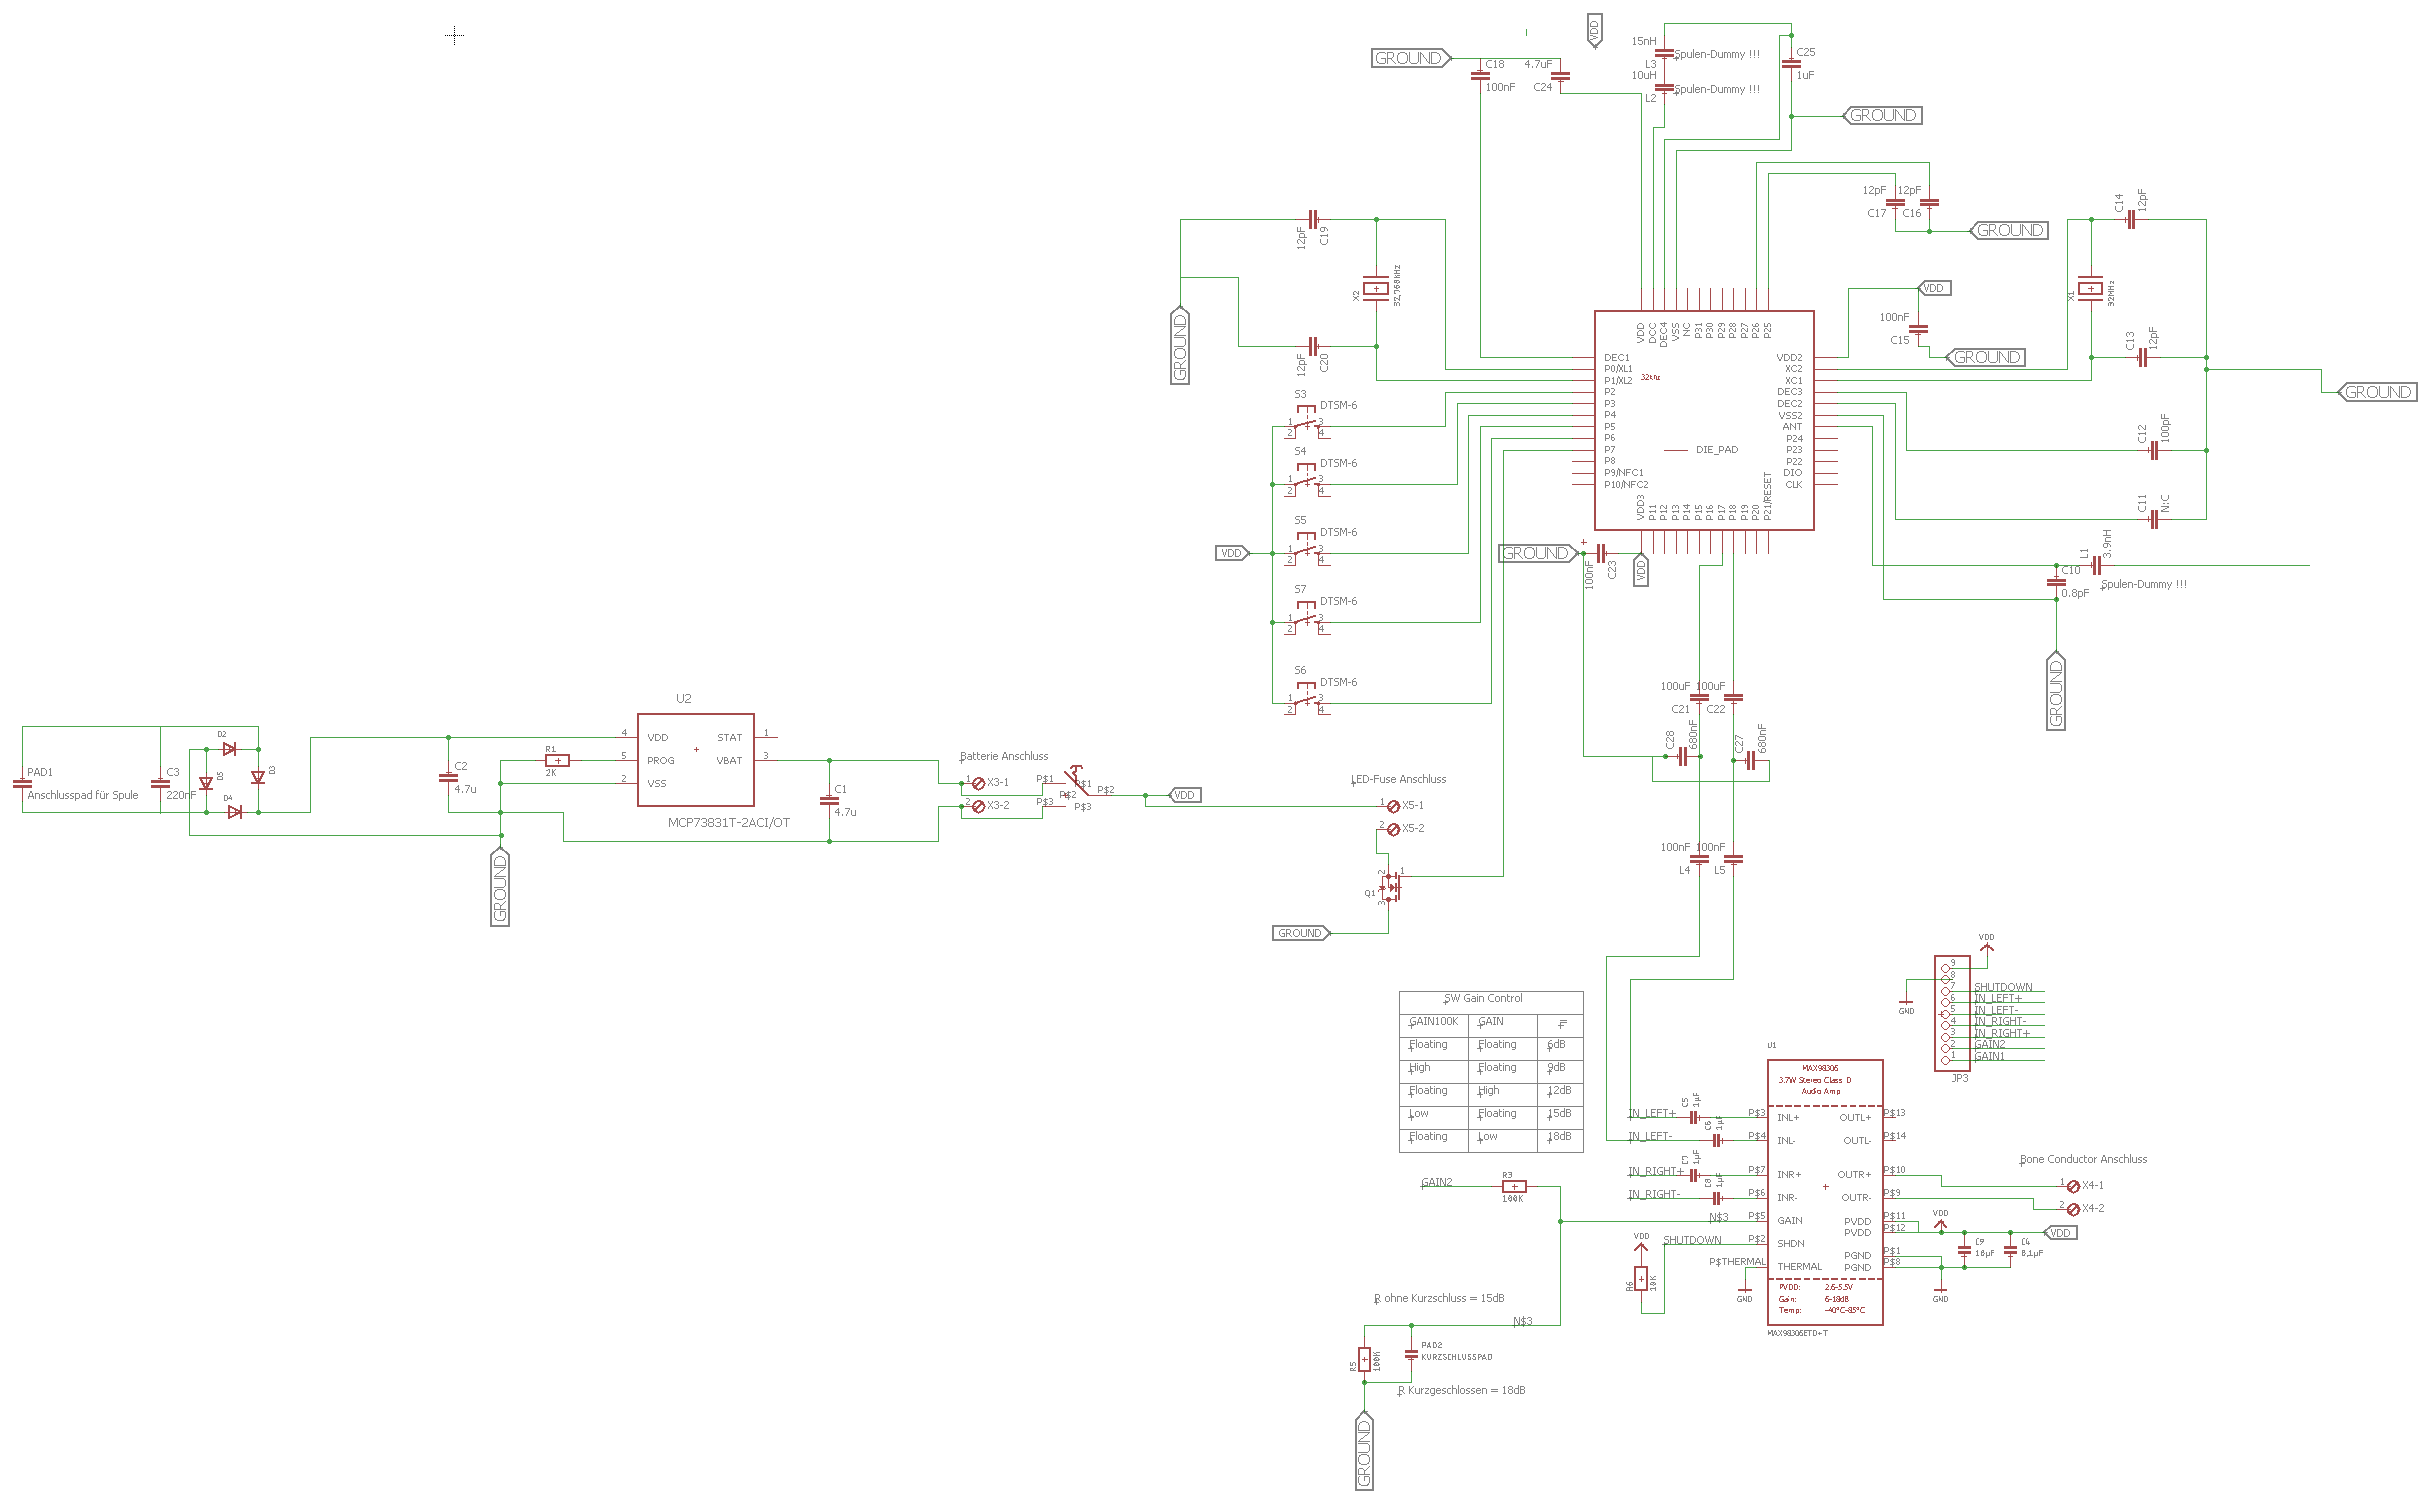
\includegraphics[width=160mm]{data/dojo-schema.png}
		\caption[das komplette Schema des Dojos]{das komplette Schema des Dojos} %picture caption
		\label{fig:dojo-schema}
	\end{center}
\end{figure}

Es ist zu sehen, dass die Ladeschaltung mit der Batterie verbunden ist. Diese Wiederrum ist mit dem Mikrokontroller und dem Verstärker verbunden, um ihre Spannungsversorgung zu gewährleisten.


- In einem weiteren Schritt würde ein Print für in den Dojo gefertigt. Dieser müsste natürlich wesentlich kleiner sein als dessen Prototyp, damit dieser in den Dojo hineinpasse. Somit wurde mit dem Layout-Programm Autocad EAGLE ein Layout erstellt, welches fünf Layer besitzt. Die Aussenmasse betragen $17mm$ auf $56mm$ auf $2mm$. Auf dem Top Layer (Layer $1$) wurde die Ladeschaltung und der Verstärker samt Filter platziert. Desweiteren sind die  hardwarespezifische Anschlüsse für die Batterie, den Knochenschallgeber und die Led-Fuseder sowie die fünf Knöpfe ebenfalls auf dem Top Layer. Dies ist damit zu begründen, da diese Subsysteme sehr kleine Ausmasse haben und deshalb effizient platziert werden konnten. Auf dem Bottom Layer (Layer $5$) ist der Komplette Mikrokontroller untergebracht, da dieser aufgrund seiner vielen externen Komponenten mehr Platz benötigt. Desweiteren gilt zu beachten dass bei diesem auf verschiedenste Schematischen Regeln geachtet werden muss, was die Platzierung noch weiter einschrenkte. Auf Layer $3$ wurde die Massefläche untergebracht, damit diese von beiden Aussenlayern gleich weit entfernt ist und somit nicht unnötig lange Masseanschlüsse für einen der beiden Seiten entsteht. Layer $4$ und $5$ dienen als zusätzliche Layer um die Verbindungen der Komponenten auf diesem engen Raum zu ermöglichen. Das finale Layout ist in dieser Abbildung \ref{fig:dojo_layout} zu sehen .
\begin{figure}[H]
	\begin{center}
		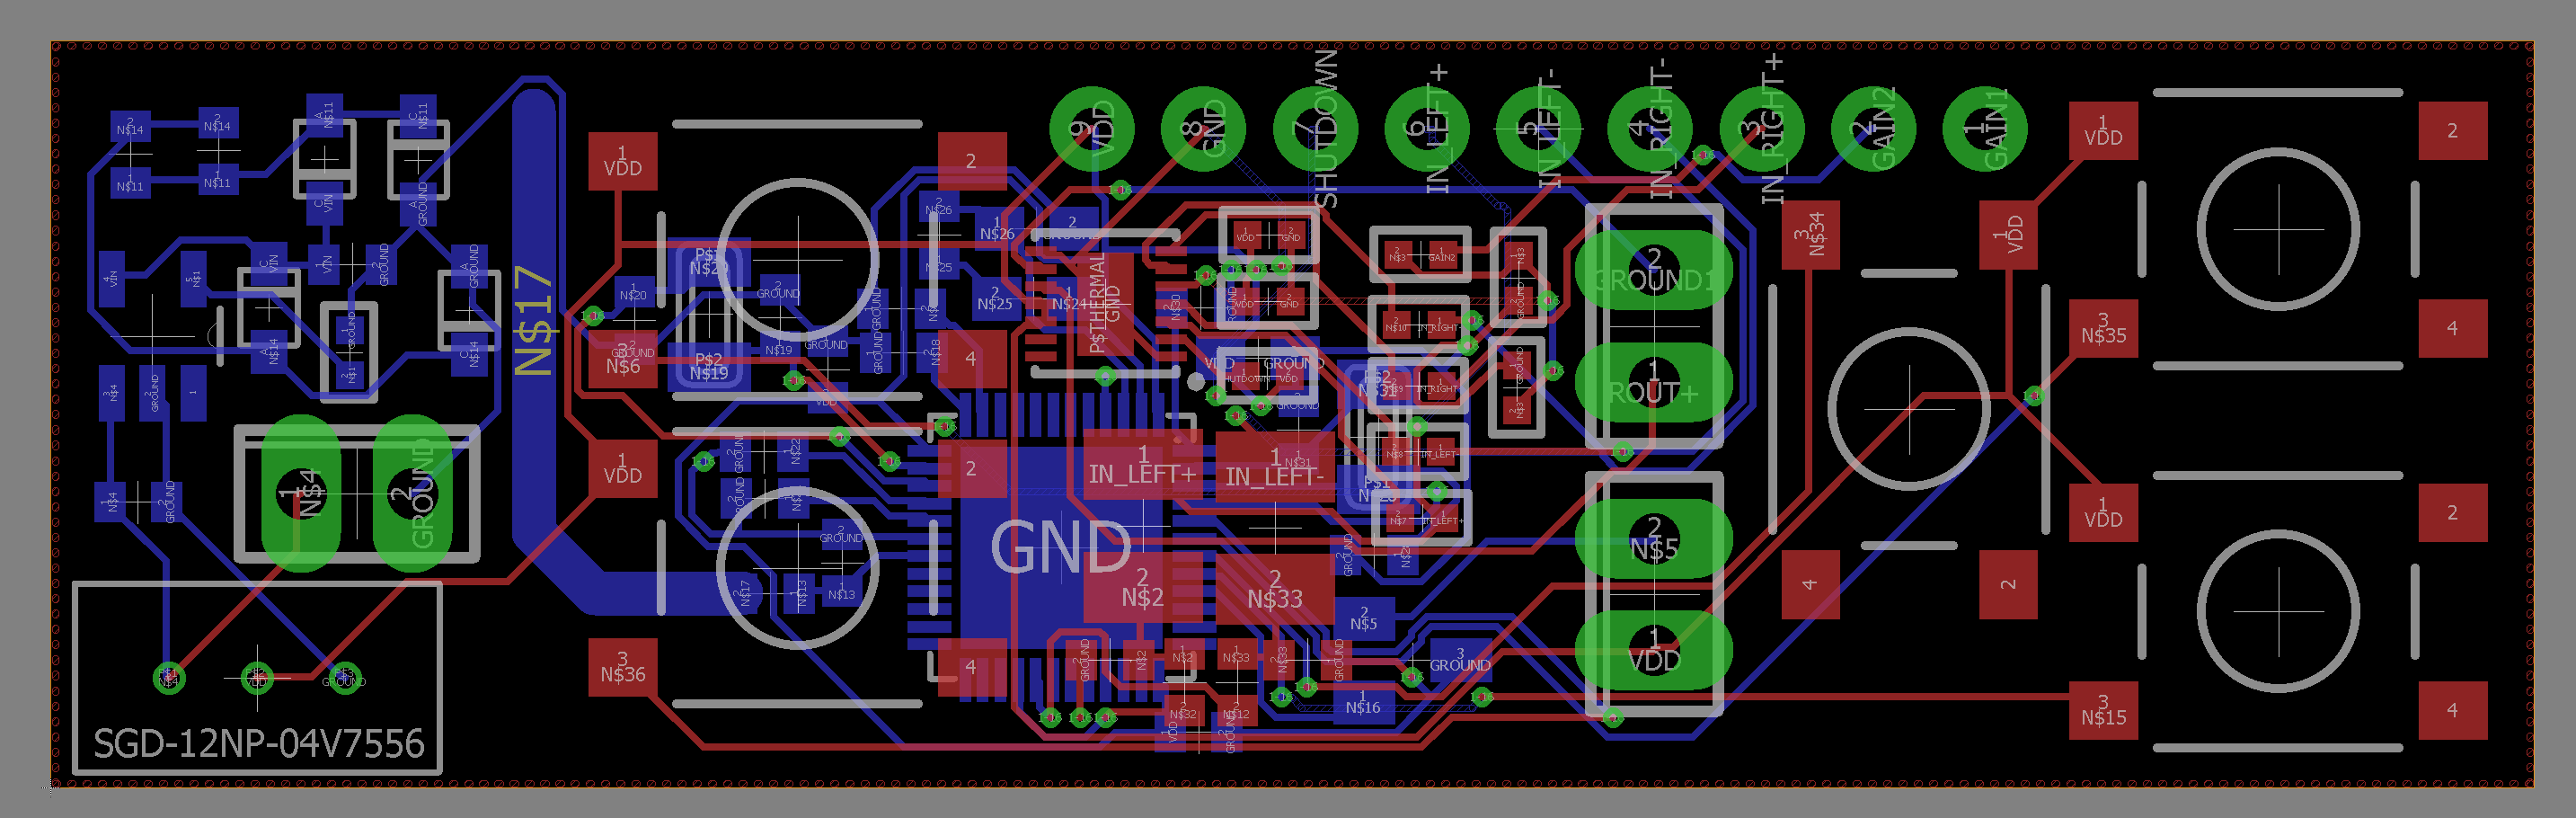
\includegraphics[width=160mm]{data/dojo_layout.png}
		\caption[Das Schema um alle Subsysteme im Dojo unterzubringen]{Das Schema um alle Subsysteme im Dojo unterzubringen} %picture caption
		\label{fig:dojo_layout}
	\end{center}
\end{figure}

Dieser Print wird im innerern des Dojos unterhalb des Bedienfeldes eingebaut. Somit können dessen Knöpfe direkt auf die Knöpfe des Printes drücken. Zusätzlich wird seitlich am Dojo ein kleiner Spalt für den Hauptschalter sein. Dieser ermöglicht zusätzliches Energiesparen wärend der Dojo nicht gebraucht wird und garantiert ein reibungsloses Laden dessen. Unterhalb des Prints wird die Batterie platziert. Somit liegt dieses, im Verhältniss schwere Bauteil, in der Hand des Trägers, was den Schwerpunkt absenkt und so zu einem angenehmeren Tragen beiträgt. Am Boden der Batterie wird die Ladespule befesstigt. Dadurch dass die Batterie lose im inneren des Gehäuses liegt wirkt diese beim Laden als anpressgewicht für die Spule.(Da der Dojo beim Laden aufrecht steht.) Somit ist gewährleistet, dass die Spule immer schön gerade am Boden aufliegt, falls diese durch das herumtragen des Dojos verrutscht sein sollte. 

Auf der gegenüberligenden seite des Dojos (also oberhalb des Prints) wird der Knochenschallsensor an der Gehäusewand montiert, damit diese die Schwingunged des Knochenschallsensors auf den Benutzer übertragen kann.